\documentclass[conference]{IEEEtran}
\IEEEoverridecommandlockouts
\usepackage{cite}
\usepackage{amsmath,amssymb,amsfonts}
\usepackage{graphicx}
\usepackage{textcomp}
\usepackage{booktabs}
\usepackage{multirow}
\usepackage{tipa}
\usepackage{xcolor}
\usepackage{tikz}
\usetikzlibrary{positioning,arrows.meta,shapes.geometric,fit,calc,backgrounds}
\usepackage[T1]{fontenc}
\newcommand{\tbd}[1]{\textcolor{red}{[TBD: #1]}}
\newcommand{\ipa}[1]{/#1/}

\begin{document}

\title{SeeSound: A Dual-Interface Prototype for Visual Guidance and Assessment of English Consonant Production by Deaf and Hard-of-Hearing Learners\\
\tbd{working title; the claim is technical feasibility, not learning effectiveness}}

\author{\IEEEauthorblockN{Kiet Pham}
\IEEEauthorblockA{\textit{\tbd{department}} \\
\textit{National Formosa University}\\
tuankiet.work.2909@gmail.com}
\and
\IEEEauthorblockN{Quang Nguyen}
\IEEEauthorblockA{\textit{\tbd{department}} \\
\textit{National Formosa University}\\
nmq.brian@gmail.com}
\and
\IEEEauthorblockN{Hui-Kai Su}
\IEEEauthorblockA{\textit{\tbd{department}} \\
\textit{National Formosa University}\\
\tbd{email}}
}

\maketitle

\begin{abstract}
\normalfont\mdseries
Deaf and hard-of-hearing (DHH) learners may have limited access to auditory feedback when they practise English consonants. This paper describes SeeSound, a web-based prototype for eight English consonants with two connected interfaces. The learner application combines articulation illustrations, camera-based lip cues, live acoustic guidance for selected sounds, and feedback after each attempt (``correct'', ``almost'', ``not yet''). A companion application lets researchers and teachers inspect recordings, spectrograms, acoustic measures, recogniser outputs, and logs. Assessment follows three routes according to the task: recogniser-assisted analysis of fricatives in single words, CTC-based goodness-of-pronunciation (GOP) scoring for stops, nasals, and the affricate, and duration-based assessment of sustained \ipa{s} and \ipa{\textesh} practice. The technical evaluation uses native speech from CMU ARCTIC and human-annotated learner speech from L2-ARCTIC. On L2-ARCTIC, the recogniser-assisted fricative route reduced the false rejection of correctly produced \ipa{s} and \ipa{\textesh} from 45\% and 43\% (fixed thresholds) to 8\% and 3\%, while detecting 100\% and 88\% of the annotated substitutions. A live centre-of-gravity indicator separated \ipa{s} from \ipa{\textesh} with an AUC of 0.86 on four adult voices, against 0.92 for the offline measure. The GOP route and the sustained-fricative route have not yet been evaluated against independent labels, and no DHH learner has used the system. The prototype is intended to support independent pronunciation practice by DHH children after initial guidance and as part of teacher-led intervention; its usability and educational effectiveness remain to be established.
\end{abstract}

\begin{IEEEkeywords}
assistive technology, deaf and hard-of-hearing, pronunciation feedback, visual feedback, phone recognition
\end{IEEEkeywords}

\section{Introduction}
Learning to produce English consonants can be challenging for DHH learners when auditory feedback is difficult to access. Although hearing devices can improve access to speech, production difficulties may remain. Ertmer and Goffman~\cite{ertmer2011}, for example, found lower accuracy and greater variability in young cochlear implant users than in typically developing peers, particularly for later-emerging consonants, and the importance of high-frequency audibility for the speech and language development of children with hearing loss has been discussed for some time~\cite{stelmachowicz2004}. These findings concern early speech development rather than English as a foreign language, but they motivate the investigation of additional feedback channels for pronunciation practice. Visual feedback offers one way to make aspects of speech production available for inspection when listening alone is insufficient.

For such feedback to support practice, learners need to understand both what the display represents and how to respond to it. Hitchcock et al.~\cite{hitchcock2023} emphasise the importance of understanding acoustic representations, selecting appropriate targets, and providing suitable guidance when using visual--acoustic biofeedback. The needs of learners and educators therefore deserve separate consideration. A learner may need a simple cue indicating what to do next, while a teacher or researcher may need to inspect the recording, the measurements, and the basis of an assessment. The PTeacher project illustrates the value of considering both perspectives: its design drew on interviews with L2 English learners and teachers to develop personalised audio-visual corrective feedback~\cite{bu2021}. In the present study, these different needs motivate two connected interfaces with different levels of detail.

Pronunciation support also involves more than identifying an error after a recording. Learners may need guidance while establishing an articulatory posture, sustaining a consonant, or moving into the following vowel. Research on automatic corrective feedback has shown benefits for targeted pronunciation errors in immigrant learners of Dutch attending teacher-led classes~\cite{neri2006}. Those findings do not establish whether a particular visual interface is understandable or effective for DHH children, so the reliability of the assessment and the usability of the guidance remain separate questions. Fixed acoustic thresholds may also respond differently across speakers and recording conditions, which makes it necessary to examine how feedback decisions are produced and where they become uncertain.

This paper presents SeeSound, a web-based prototype for eight English consonants: \ipa{s}, \ipa{\textesh}, \ipa{f}, \ipa{t\textesh}, \ipa{m}, \ipa{n}, \ipa{p}, and \ipa{b}. Its learner application combines articulation illustrations, camera-based lip cues, and live acoustic guidance for selected sounds with feedback after each attempt. A companion application allows researchers and teachers to inspect recordings, acoustic measurements, recognition outputs, and development logs. Assessment follows different routes according to the task: recogniser-assisted analysis of fricatives in words, CTC-based pronunciation scoring for stops, nasals, and the affricate, and duration-based assessment of sustained-fricative practice. The scope is word-initial consonant production and guided consonant-to-vowel practice; the camera measures visible lip movements, not tongue position.

The study makes three contributions.
\begin{enumerate}
\item It describes a prototype that presents simplified, step-by-step guidance to learners while retaining detailed analytical information for researchers and teachers.
\item It explains how live acoustic and lip cues are combined with task-specific assessment routes, and states what each route can and cannot support.
\item It reports technical evaluations and development observations, keeping corpus-based evidence, single-speaker logs, and simulated-input tests apart.
\end{enumerate}
The prototype is intended to support independent practice following initial guidance and educator-led pronunciation intervention. Its usability and educational effectiveness for DHH learners have not yet been established.

\section{Related Work}
\textit{Visual feedback for speech training.} Visual--acoustic biofeedback, in which the learner matches a live acoustic representation, such as a linear predictive coding spectrum, to a target, is an established clinical technique for residual speech sound errors, and a recent tutorial states that its success depends on the comprehension of the representation by clinician and client, on the choice of the acoustic target and template, and on the practice schedule~\cite{hitchcock2023}. These requirements motivate a display in which the learner is not required to interpret a spectrum, and in which a categorical mark accompanies the signal. Visual feedback can offer DHH learners an additional method for observing and comparing their productions with target patterns by making aspects of speech production visible~\cite{hitchcock2023}.

\textit{Consonant perception and production in DHH learners.} For listeners with hearing impairment, visual cues contribute more to the identification of consonants than of vowels~\cite{moradi2017}, and cochlear-implant (CI) users rely more strongly on the visual cue than normal-hearing listeners when the auditory cue is weak~\cite{desai2008}. CI listeners can also use visual information to accommodate the acoustic differences between \ipa{s} and \ipa{\textesh} across talkers~\cite{winn2013}, and deaf adults with CIs retain a speechreading skill that is not inferior to that of hearing adults~\cite{pimperton2017}. With respect to production, young CI recipients produce initial consonants with lower accuracy and greater variability than typically developing peers, and fricatives and affricates are acquired later than stops and nasals~\cite{ertmer2011}; word-initial fricatives have also been studied in Mandarin-speaking children with CIs~\cite{yang2017}. Collectively, these findings highlight a need for simplified visual feedback to support English consonant practice by DHH students.

\textit{Spectrographic and instrumental feedback for deaf learners.} Spectrographic displays have been used with deaf speakers for a long time. In a small single-case study with four deaf adolescents, each participant improved under both spectrographic and noninstrumental instruction, and the advantage of the spectrographic condition was limited to some participants~\cite{ertmermaki2000}. Children aged 6 to 11 years, with and without hearing impairment, recognised spectrographic cues above chance after a familiarisation period, with formant contrasts recognised more accurately than consonant manner contrasts and no difference between the two hearing groups~\cite{ertmer2004}. These studies concern small samples and displays that the learner has to interpret, so they do not settle whether a guided, step-by-step visual interface supports independent practice.

\textit{Corrective feedback and automatic detection of L2 pronunciation errors.} Acoustic--phonetic classifiers trained for specific frequently mispronounced sounds, with linear discriminant analysis and decision trees, were able to discriminate correct from incorrect productions in native and non-native speech, whereas confidence measures from speech recognisers are less accurate predictors of phone-level quality~\cite{truong2005}. Evidence for ASR-based corrective feedback comes from adult learners in teacher-led courses~\cite{neri2006}, and PTeacher combined learner and teacher interviews with exaggerated audio-visual feedback for L2 English learners~\cite{bu2021}; none of these systems targets DHH children. The present design combines both families of methods: a recogniser decides which sound was produced, and interpretable acoustic measures determine its degree. Self-supervised representations have furthermore been shown to predict the intelligibility of L2 talkers over and above traditional acoustic--phonetic cues~\cite{kim2025}, which supports the use of recogniser features for learner speech. The recogniser is a wav2vec~2.0 model~\cite{baevski2020} fine-tuned for multilingual phone recognition~\cite{xu2022}, and the acoustic characterisation of English fricatives follows the spectral-moment approach~\cite{jongman2000}. Learner errors are taken from L2-ARCTIC~\cite{zhao2018}.

\textit{Word selection.} The target words (\textit{she}, \textit{see}, \textit{fee}, \textit{pea}, \textit{bee}, \textit{me}, \textit{knee}, \textit{cheat}) are common monosyllabic words; large-scale age-of-acquisition ratings~\cite{kuperman2012} can be used to verify that they are acquired early. \tbd{Check the ratings of the eight words and report them, or drop this sentence.}

\tbd{Broaden with computer-assisted pronunciation training (CAPT) and mispronunciation-detection literature, a primary reference for goodness-of-pronunciation (GOP) scoring and CTC-based adaptations of it, and universal design for learning (UDL) in language learning; this section cites only the sources checked so far.}

\section{System Design and Implementation}
\subsection{Architecture and User Roles}
SeeSound consists of two web applications that share one scoring package (Fig.~\ref{fig:arch}). The \emph{learner application} is meant for children: a home page, an optional Sound Check, eight lessons, a lip mirror, and a page showing the stars earned. The \emph{researcher/teacher application} is a separate interface for people who need to examine why a judgement was made: it shows the recording, the spectrogram with the detected consonant, the numerical measures, the candidate scores and decoded phones of the recogniser, and the logs. Audio is recorded in the browser and sent to a local Python back end; the lip features are computed in the browser from a face-landmark model that runs offline, and only numbers are passed on. The two interfaces are deliberately separate, because a display that helps a researcher (a spectrogram, a table of cues) is not what a child needs in order to know what to do next.

\begin{figure*}[!t]
\centering
\resizebox{0.97\textwidth}{!}{%
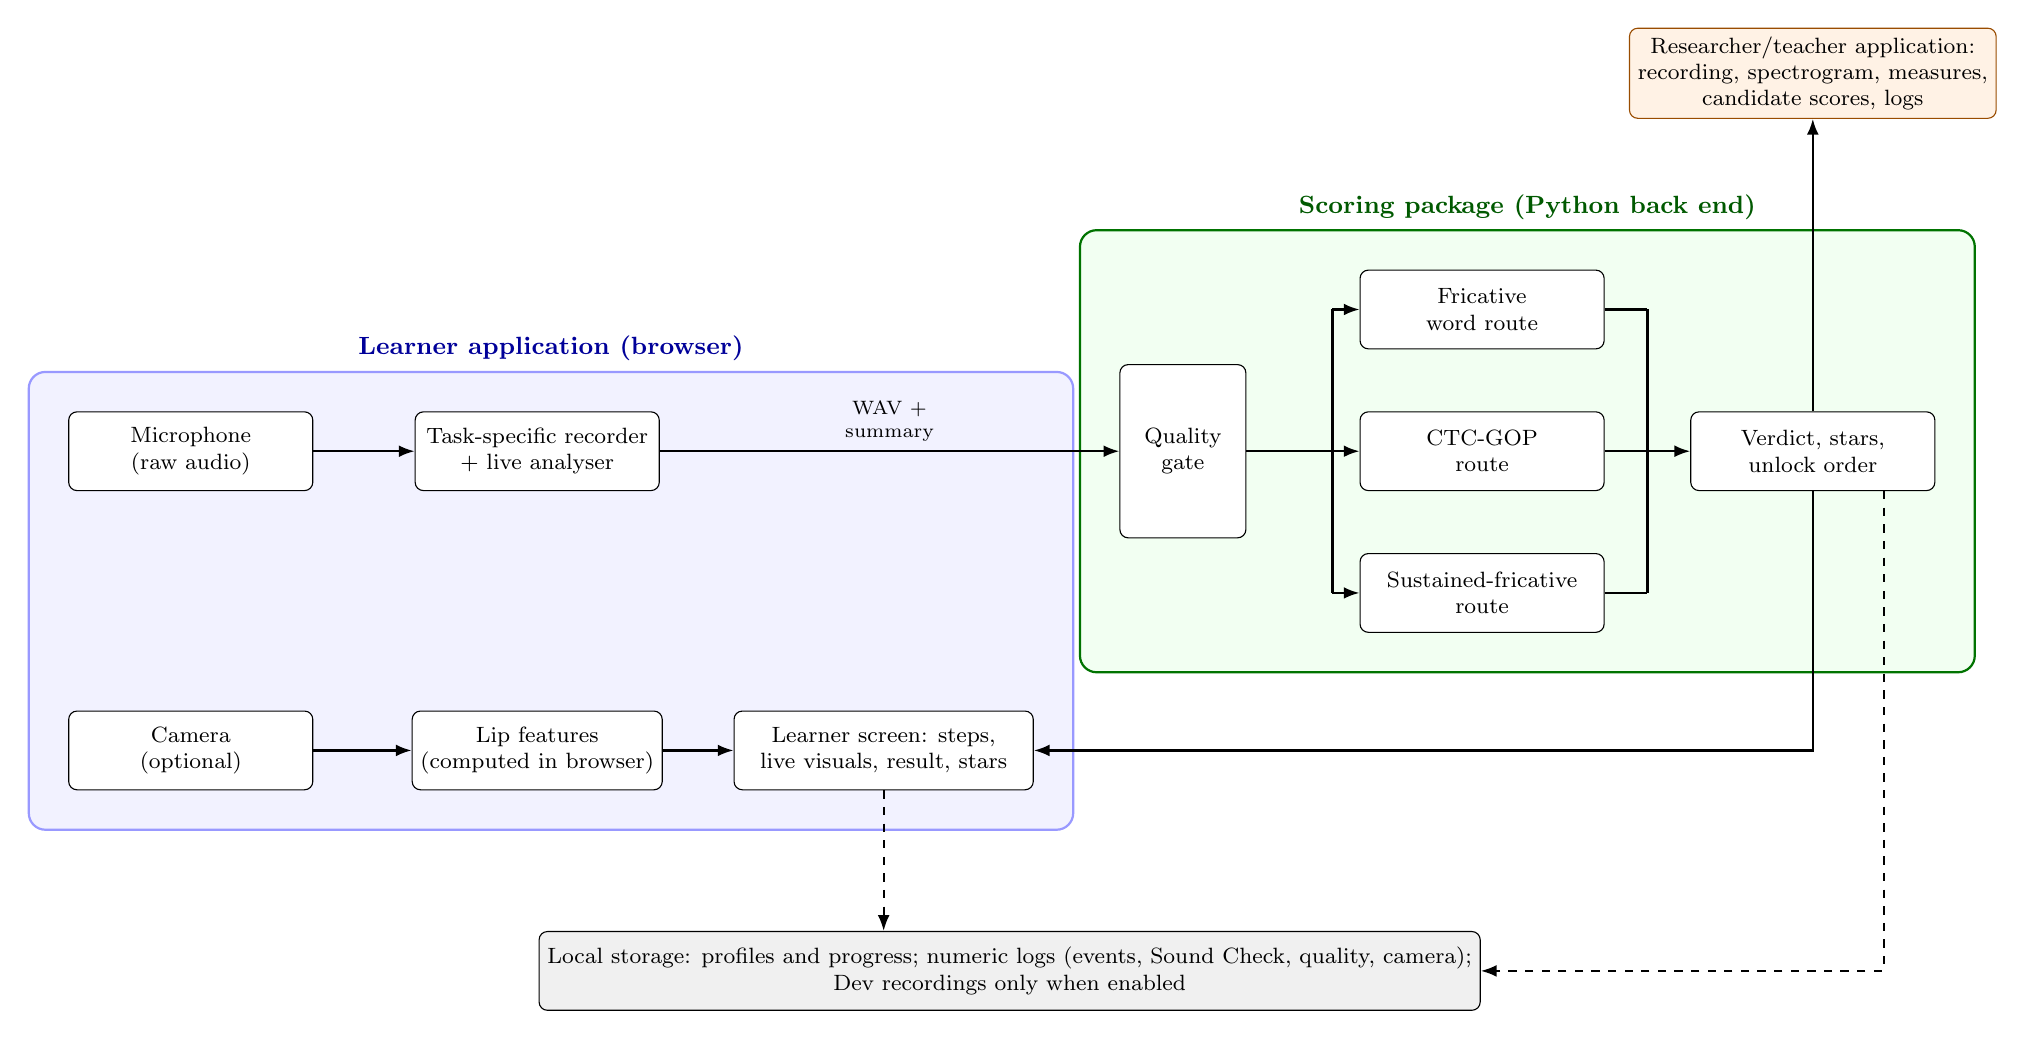
\begin{tikzpicture}[font=\footnotesize,
  box/.style={draw, rounded corners=3pt, align=center, fill=white, minimum height=10mm, minimum width=31mm, inner sep=3pt},
  grp/.style={draw, rounded corners=6pt, inner sep=5mm, thick},
  arr/.style={-{Latex[length=2mm]}, thick},
  bus/.style={thick}]
  % learner application (browser)
  \node[box] (mic) at (0,4.6) {Microphone\\(raw audio)};
  \node[box] (cam) at (0,0.8) {Camera\\(optional)};
  \node[box] (rec) at (4.4,4.6) {Task-specific recorder\\+ live analyser};
  \node[box] (lip) at (4.4,0.8) {Lip features\\(computed in browser)};
  \node[box, minimum width=38mm] (ui) at (8.8,0.8) {Learner screen: steps,\\live visuals, result, stars};
  \begin{scope}[on background layer]
    \node[grp, fill=blue!5, draw=blue!40, fit=(mic)(cam)(rec)(lip)(ui), label={[font=\small\bfseries, text=blue!60!black]above:Learner application (browser)}] (gA) {};
  \end{scope}
  % scoring package
  \node[box, minimum width=16mm, minimum height=22mm] (gate) at (12.6,4.6) {Quality\\gate};
  \node[box] (r1) at (16.4,6.4) {Fricative\\word route};
  \node[box] (r2) at (16.4,4.6) {CTC-GOP\\route};
  \node[box] (r3) at (16.4,2.8) {Sustained-fricative\\route};
  \node[box] (vd) at (20.6,4.6) {Verdict, stars,\\unlock order};
  \begin{scope}[on background layer]
    \node[grp, fill=green!5, draw=green!45!black, fit=(gate)(r1)(r2)(r3)(vd), label={[font=\small\bfseries, text=green!35!black]above:Scoring package (Python back end)}] (gB) {};
  \end{scope}
  % researcher / teacher application
  \node[box, fill=orange!10, draw=orange!60!black, minimum width=44mm] (dev) at (20.6,9.4) {Researcher/teacher application:\\recording, spectrogram, measures,\\candidate scores, logs};
  % storage
  \node[box, fill=gray!12, minimum width=100mm] (st) at (10.4,-2.0) {Local storage: profiles and progress; numeric logs (events, Sound Check, quality, camera);\\Dev recordings only when enabled};
  % arrows
  \draw[arr] (mic) -- (rec);
  \draw[arr] (cam) -- (lip);
  \draw[arr] (lip) -- (ui);
  \draw[arr] (rec.east) -- node[above, font=\scriptsize, align=center]{WAV +\\summary} (gate.west |- rec.east);
  \coordinate (b1) at (14.5,4.6);
  \draw[bus] (gate.east) -- (b1); \draw[bus] (b1 |- r1) -- (b1 |- r3);
  \draw[arr] (b1 |- r1) -- (r1.west); \draw[arr] (b1) -- (r2.west); \draw[arr] (b1 |- r3) -- (r3.west);
  \coordinate (b2) at (18.5,4.6);
  \draw[bus] (r1.east) -- (b2 |- r1); \draw[bus] (b2 |- r1) -- (b2 |- r3); \draw[bus] (r3.east) -- (b2 |- r3);
  \draw[bus] (r2.east) -- (b2); \draw[arr] (b2) -- (vd.west);
  \draw[arr] (vd.north) -- (vd.north |- gB.north) -- (dev.south |- gB.north) -- (dev.south);
  \draw[arr] (vd.south) |- (ui.east);
  \draw[arr, dashed] (ui.south) -- (ui.south |- st.north);
  \draw[arr, dashed] ([xshift=9mm]vd.south) |- (st.east);
\end{tikzpicture}}
\caption{System architecture. The learner application records audio and, if the user switches it on, computes lip features in the browser (no camera picture is stored or sent). The shared scoring package checks the recording quality and then follows one of three routes according to the task. The researcher/teacher application reads the same recordings and scores. Dashed arrows: data written to the local machine.}
\label{fig:arch}
\end{figure*}

\subsection{Learner Workflow}
The learner chooses or creates a profile, may run Sound Check (Section~\ref{sec:soundcheck}), and then opens a lesson (Fig.~\ref{fig:flow}). A lesson shows the word with a picture for its meaning and a picture for the sound, an articulation illustration with the steps of the movement, a recorder with live feedback, and, for seven of the eight sounds (all but \ipa{f}), an optional lip mirror. All text is shown in English and Traditional Chinese. After a recording, the recorder is replaced by the result: a three-level mark (\textit{correct}, \textit{almost}, \textit{not yet}), a written tip, and one to three stars. A profile keeps the best result for each word; stars are taken from the colour and the closeness of the result (three for green, two or one for yellow, none for red). The lessons are ordered \textit{she}, \textit{see}, \textit{fee}, \textit{pea}, \textit{bee}, \textit{me}, \textit{knee}, \textit{cheat}, and a lesson opens when the one before it has at least two stars; when no profile is chosen, every lesson is open and nothing is saved. This order and the pass line of two stars are application rules chosen during development, not a validated sequence of difficulty or a certificate of mastery. Sound Check is offered but not required.

\begin{figure*}[!t]
\centering
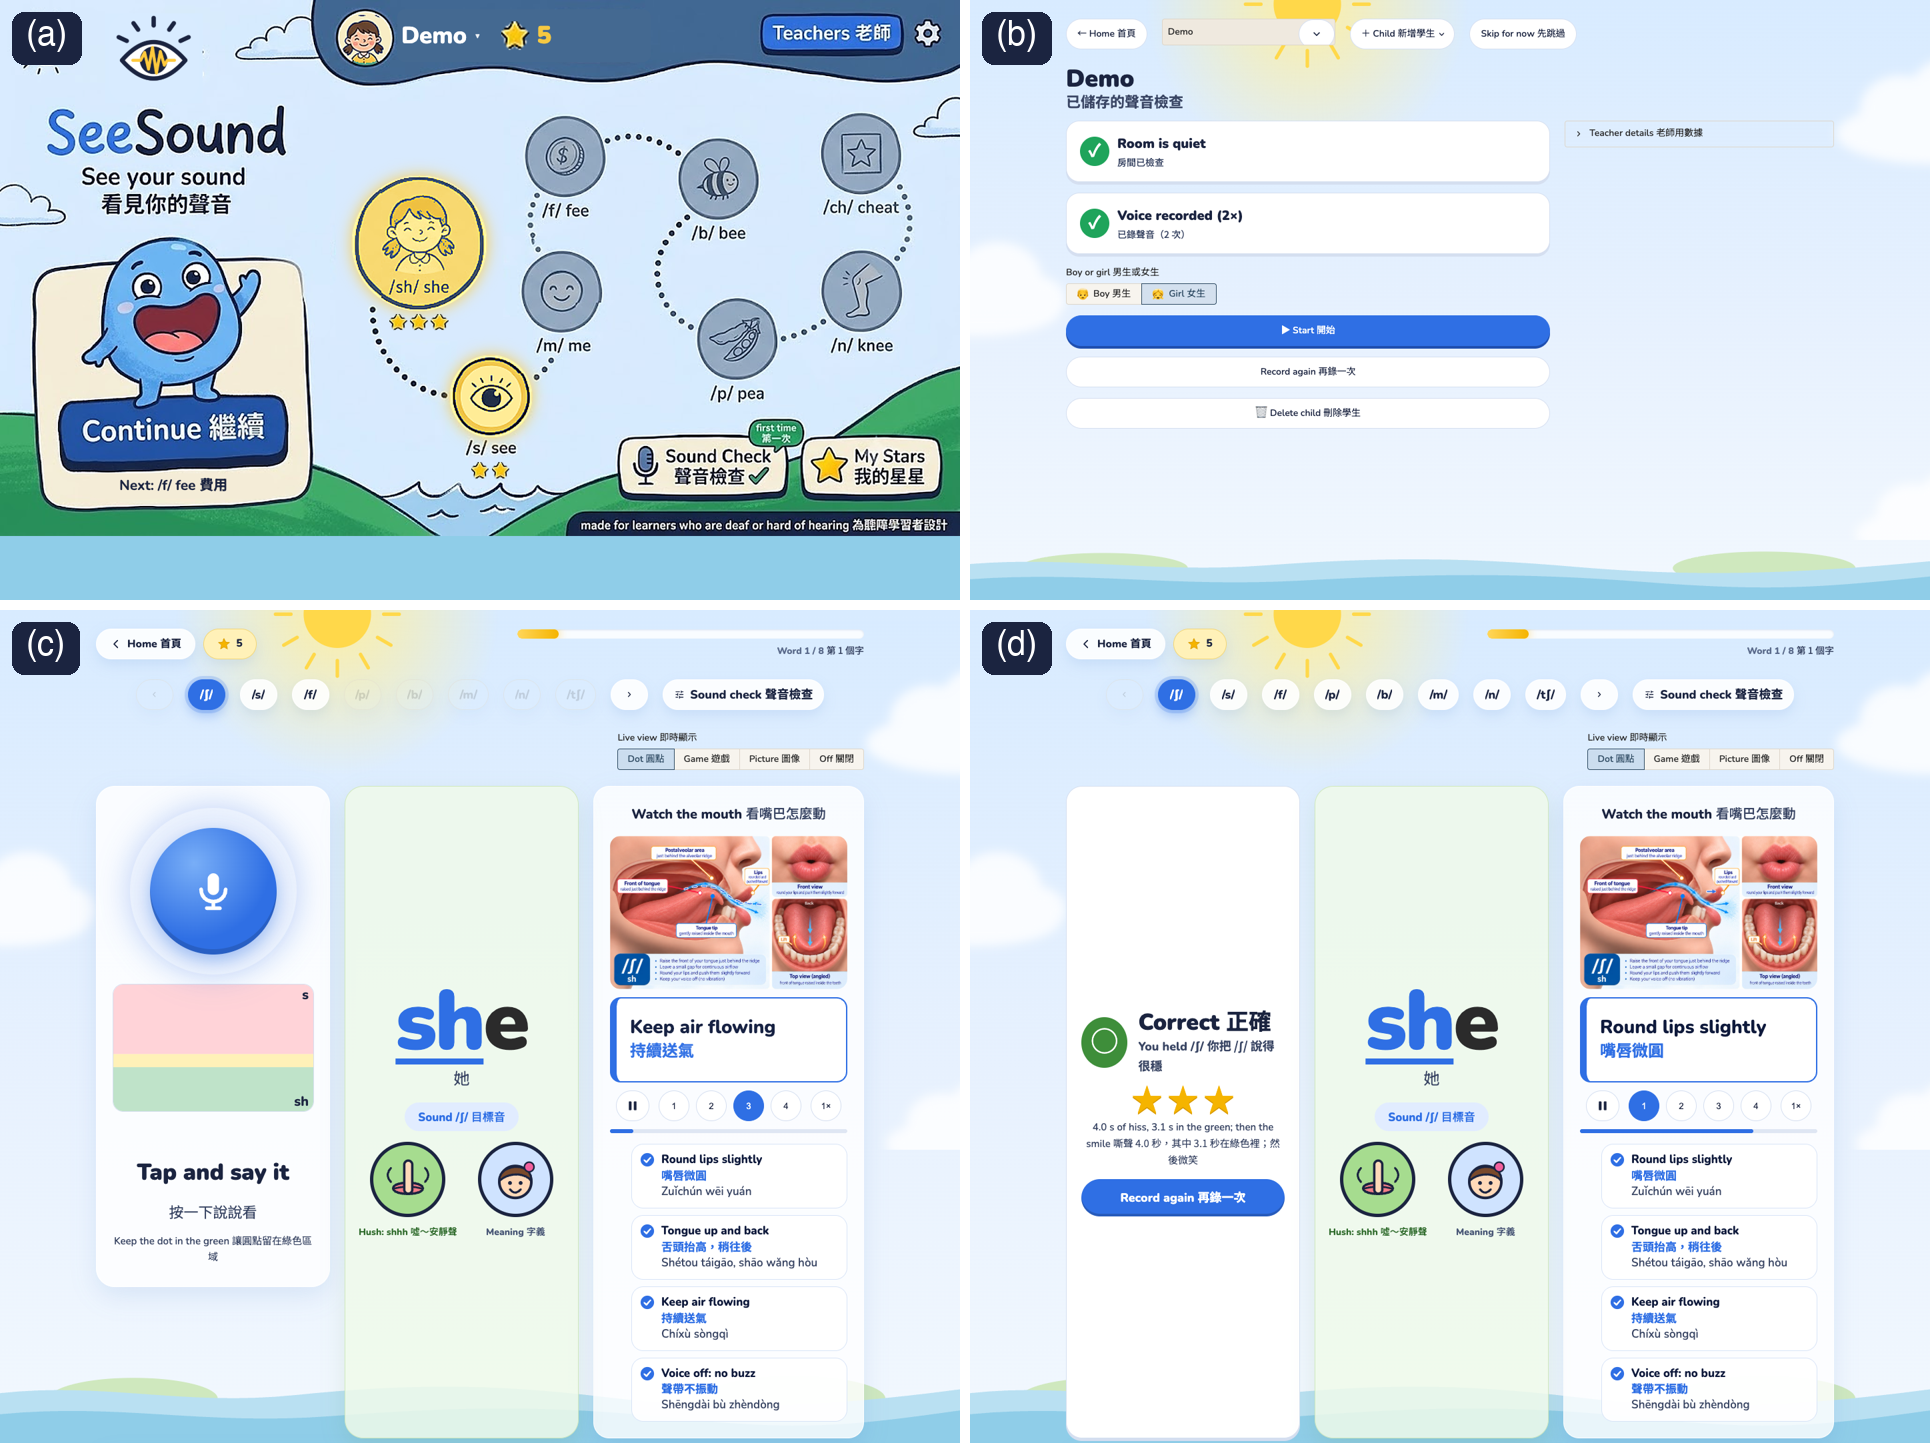
\includegraphics[width=0.96\textwidth]{figs/fig_learner_flow.png}
\caption{The learner application as run for this paper, with a test profile (name chosen for the figure) and a synthetic microphone signal. (a)~Home page with the stars earned and the next sound. (b)~Saved Sound Check of the profile. (c)~Lesson for \textit{she}: recorder with the live zone display, word card, and the articulation steps. (d)~Result after a sustained hiss: mark, three stars, and the time spent in the target zone.}
\label{fig:flow}
\end{figure*}

\subsection{Recording and Live Guidance}
Audio is recorded with a component written for the application, which requests the microphone with echo cancellation, noise suppression, and automatic gain control switched off, decodes the browser recording, and sends mono 16-bit WAV to the back end. In the first development recordings the default browser processing clipped the signal, removed the weak onset of \ipa{b}, and left the recogniser hearing \ipa{m} instead; switching it off removed these effects but exposed the background noise. This choice was made on the basis of the recordings of one adult and one microphone, and it may not be best for every device or room.

The recording rules differ between tasks (Table~\ref{tab:tasks}). The word recorder used for \ipa{f}, \ipa{p}, and \ipa{b} stops after three seconds. The guided recorders listen to the room for 0.6~s after the tap and set their sound gate from it; they then follow the stages of the task and stop when the child has been silent for 1.5~s, when the task is complete, or after a maximum of 10--12~s. For \ipa{s} and \ipa{\textesh}, the child holds the hiss for at least 0.4~s inside the target zone shown by a moving dot (or a game, or a scrolling spectrogram) and then smiles into the following ``ee''; for \ipa{m} and \ipa{n}, the child hums and then moves to a vowel; for \ipa{t\textesh}, a train scene follows the pop, the hiss, and the voice. Fig.~\ref{fig:live} shows three of these displays during a recording. Before scoring, every recording passes a quality gate that refuses recordings that clip, are too quiet, or lie less than 12~dB above their own background (a limit lowered from 20~dB after the first real recordings, and not validated for children).

\begin{figure}[!t]
\centering
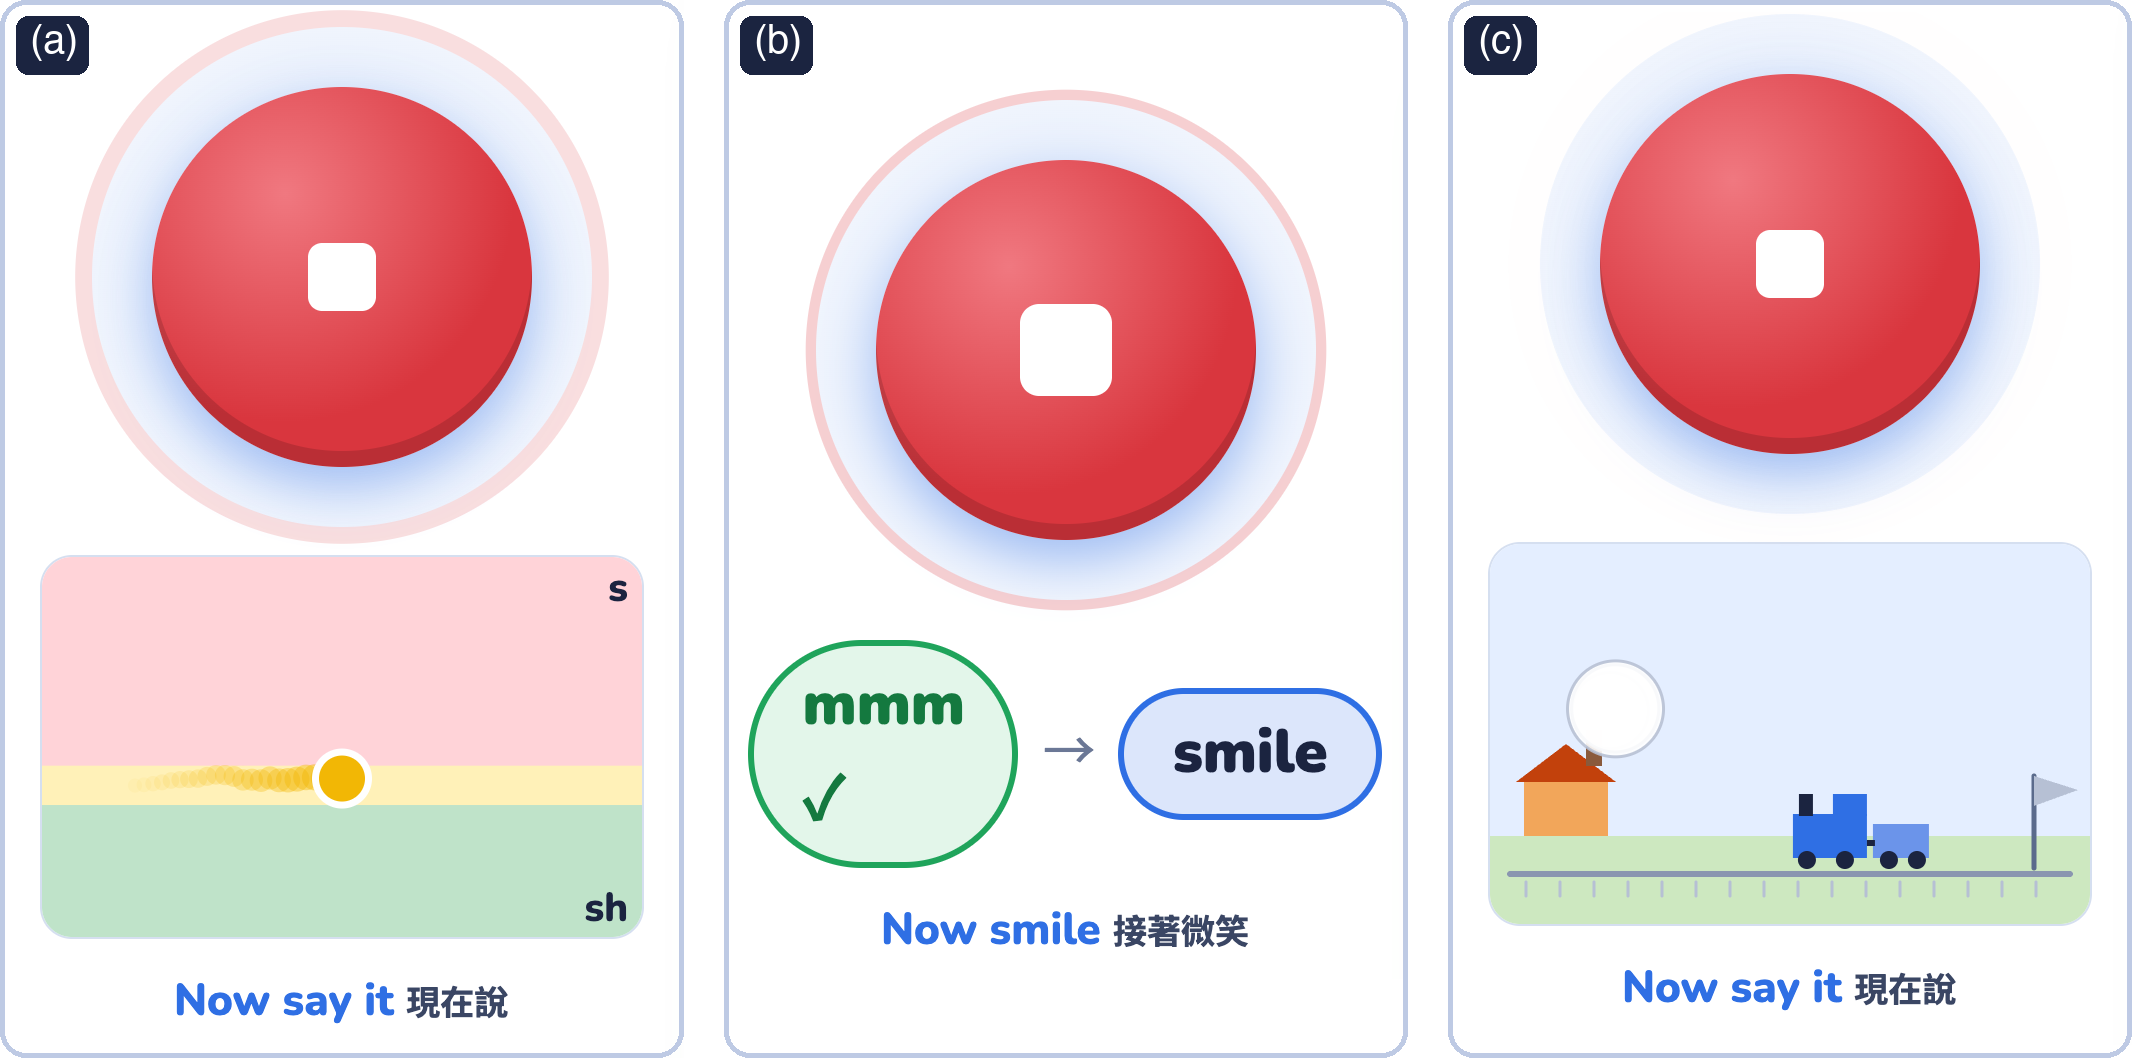
\includegraphics[width=\columnwidth]{figs/fig_live.png}
\caption{Live guidance during a recording (red button), driven by synthetic audio played into the browser. (a)~\ipa{\textesh}: the dot has moved from the \ipa{s} side into the yellow band while a hiss is held. (b)~\ipa{m}: the hum was detected (tick) and the next step, the smile, is shown. (c)~\ipa{t\textesh}: the train reacts to the pop, the hiss, and the voice.}
\label{fig:live}
\end{figure}

\begin{table*}[!t]
\caption{Sounds, tasks, and the current assessment route. Words are those of the lessons. ``Camera cue'': what the lip mirror checks; the camera does not see the tongue or the airflow.}
\label{tab:tasks}
\centering
\footnotesize
\begin{tabular}{p{1.5cm}p{3.6cm}p{3.0cm}p{2.4cm}p{4.5cm}}
\toprule
Sound (word) & Live guidance & Camera cue & Recording & Assessment route \\
\midrule
\ipa{\textesh} (\textit{she}), \ipa{s} (\textit{see}) & Dot, game, or scrolling spectrogram; hold the hiss in the zone for 0.4~s, then ``ee'' & Three-step ghost mouth (lips rounded or spread, then smile) & Guided, stops on silence or task end & Sustained-fricative route (live summary); word route when no summary is available \\
\ipa{f} (\textit{fee}) & Level meter relative to the child's ``aaa'' & None & 3~s & Fricative word route \\
\ipa{p} (\textit{pea}), \ipa{b} (\textit{bee}) & None while speaking & Lips closed, then open, then spread; camera only & 3~s & CTC-GOP \\
\ipa{m} (\textit{me}), \ipa{n} (\textit{knee}) & Hum, then vowel; coach combining voice and lips & Lips closed (\ipa{m}) or slightly open (\ipa{n}), then smile & Guided, stops after the vowel or on silence & CTC-GOP \\
\ipa{t\textesh} (\textit{cheat}) & Train: pop, hiss, voice & Three-step ghost mouth & Guided & CTC-GOP, plus two lamps (pop slope, hiss length) \\
\bottomrule
\end{tabular}
\end{table*}

\subsection{Camera-Based Lip Cues}
When the user switches the lip mirror on, a face-landmark model~(MediaPipe Face Landmarker, run in the browser from local files) reads each camera frame. Only two ratios are used: the gap between the inner upper and lower lip, and the distance between the mouth corners, each divided by the distance from forehead to chin. The lips count as together when the gap ratio is below 0.03 (with a margin to avoid flicker); a smile is counted when the mouth width is at least 1.03 times the width of the same child's closed lips while the gap stays below 0.10; \ipa{n} asks for a gap between 0.03 and 0.12. For \ipa{s}, \ipa{\textesh}, \ipa{t\textesh}, \ipa{p}, and \ipa{b}, a ghost mouth shows the shape of each step as a target. These limits and shapes are first guesses made on one adult face; they have not been tuned on children's faces, glasses, or poor light. The camera picture is not shown, stored, or sent anywhere, and the mirror runs only when switched on. During development, numbers about the lips and the sound (not the picture or the voice) were written to a local log.

\subsection{Researcher and Teacher Application}
The second application offers record or upload, the spectrogram with the detected consonant and an adjustable boundary, the numerical measures, a comparison with reference voices, the candidate scores and decoded phones of the recogniser, a log of recordings that can be listened to, flagged, and deleted, and plots of the camera and microphone numbers over time (Fig.~\ref{fig:dev}). It does not manage classes or students.

\begin{figure}[!t]
\centering
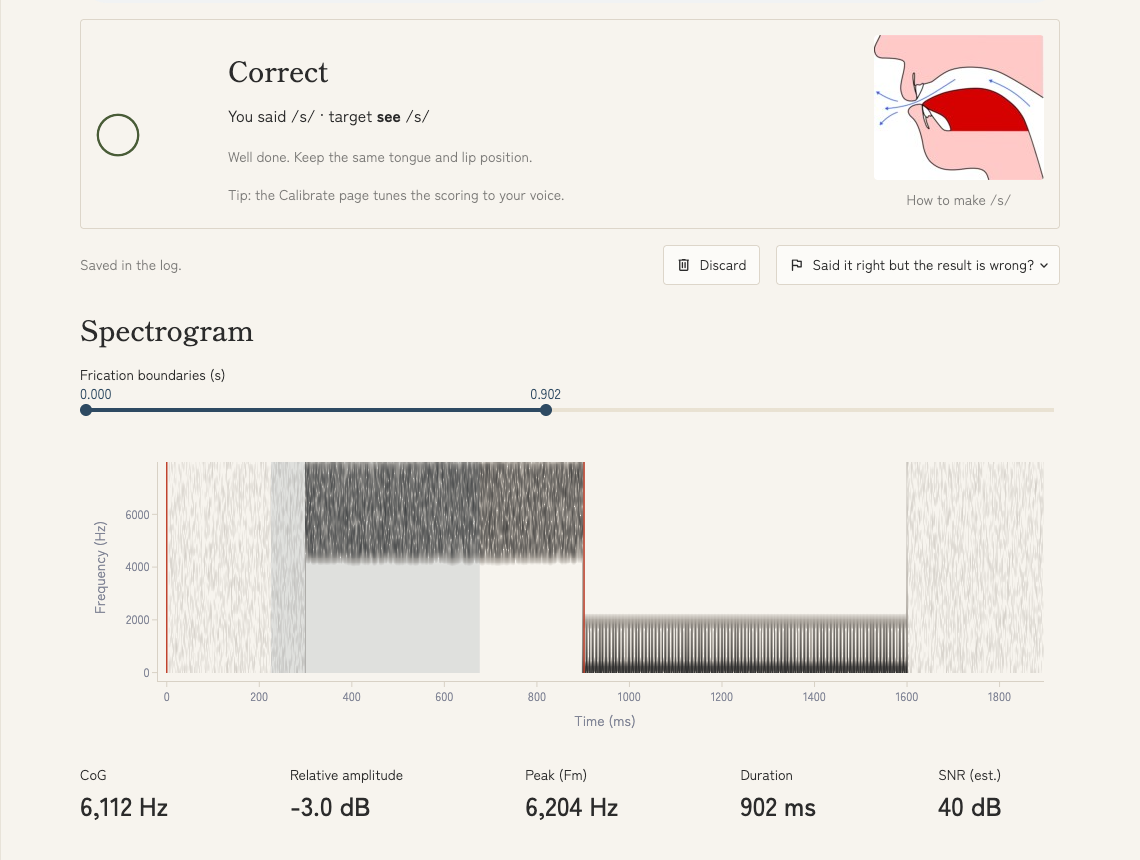
\includegraphics[width=\columnwidth]{figs/fig_dev.png}
\caption{Researcher/teacher application with a synthetic test recording (a band-limited noise followed by a voiced vowel, uploaded as \textit{see}): verdict, spectrogram with the detected fricative, measures, and the cues used by the rules.}
\label{fig:dev}
\end{figure}

\subsection{Data Handling}
Profiles hold a name, a boy/girl choice used for the picture on the home page, the Sound Check numbers, and the stars; none of them is shown in this paper's figures. The learner application writes numbers and choices only: one line per lesson opening, attempt (what was scored and why, the stars, the quality numbers, the live summary), and retake, and one line each time a Sound Check is saved, repeated, or deleted, together with the numbers it replaced. It does not keep the child's audio; the researcher/teacher application keeps recordings only when its log is switched on. All files stay on the local machine. Before use with children, consent, storage, and deletion procedures have to be defined \tbd{ethical approval and procedures}.

\section{Signal Processing and Assessment}\label{sec:assess}
\subsection{Sound Check and Voice-Size Scaling}\label{sec:soundcheck}
Sound Check measures the room (three seconds of silence) and asks the child to say a long ``aaa'' twice. The median third formant of the vowel, divided by a reference of 2625~Hz, gives a factor limited to 0.85--1.5 that shifts the \ipa{s}--\ipa{\textesh} boundary (the \ipa{f} meter uses the level of the same ``aaa'' instead); the child is never asked to say the sound being learned. The factor was checked on synthetic vowels only, so it is a provisional scaling and not a validated vocal-tract normalisation. The reference value was set from memory of published adult formant averages and has to be confirmed. The researcher/teacher application keeps an older calibration with six recordings of \textit{see}, \textit{she}, and \textit{fee}.

\subsection{Consonant Location and Acoustic Measures}
For fricatives, the onset is the start of the run of high-band energy (2.5--12~kHz) that precedes the vowel, with a frame counted as part of the run when it lies at least 15~dB above the noise floor of the recording itself, and the offset is the first voiced frame. The centre of gravity (CoG) is computed on the middle 50\% of this segment with a rectangular window and a spectral power of two, which is the setting of the manual Praat measurements used as reference. The hiss level relative to the following vowel separates \ipa{f} from the sibilants. For \ipa{p} and \ipa{b}, the voice onset time (VOT) is the interval between the burst, detected in the 1.5--7.5~kHz band, and the first voiced frame; this rule is kept for the researcher application. For the live dot, the CoG is weighted by power between 2 and 8~kHz and smoothed over frames; its zones are \ipa{\textesh} below 3940~Hz and \ipa{s} above 4540~Hz, before the voice-size factor, with a yellow band in between.

\subsection{Fricative Word Route}
A multilingual phone recogniser (wav2vec~2.0 XLSR-53 fine-tuned on eSpeak phone transcriptions~\cite{baevski2020,xu2022}) is applied to the segment located above. The posterior probabilities of the phones belonging to each sound class are averaged over the consonant, and the class with the highest mean posterior is taken as the sound heard. The design principle is a division of labour: the recogniser decides whether the intended sound was produced, whereas the acoustic measures decide between \textit{correct} and \textit{almost}. When the recogniser hears a different sound, the verdict is \textit{not yet}; when it hears the intended sound but the thresholds disagree, the verdict is \textit{almost}. A gate based on the first decoded phone withholds scoring when a different kind of sound (for example, a fricative for a stop target) is heard. When the child has calibrated, every feature can be expressed relative to the child's six calibration recordings, and a shrinkage linear discriminant model trained on eight native voices estimates the probabilities of \ipa{s}, \ipa{\textesh}, and a weak hiss; this part is optional. The route is used for \ipa{f}, for \ipa{s} and \ipa{\textesh} in single words, and in the researcher application.

\subsection{CTC-Based GOP Route}\label{sec:gop}
For \ipa{p}, \ipa{b}, \ipa{m}, \ipa{n}, and \ipa{t\textesh}, the verdict is a goodness-of-pronunciation score computed from the CTC output of the same recogniser, so that no calibration to the learner is needed. The log-posteriors are computed for the whole recording (one frame per 20~ms). The first frame whose blank probability is below 0.9 marks the onset, and a window of 22 frames (about 0.45~s) starting three frames before it is analysed. For each candidate consonant $c$ of a confusable set and each single vowel $v$ of the recogniser's vocabulary, the CTC log-likelihood of the sequence $[c,v]$ is computed, and the likelihoods are summed over vowels and over spelling variants of $c$, so that the vowel the learner chose does not matter in the computation:
\begin{equation}
P(c)=\frac{L(c)}{\sum_{c'} L(c')},\qquad L(c)=\sum_{v}\sum_{c_i\in V(c)} p_{\mathrm{CTC}}\bigl([c_i,v]\bigr),
\end{equation}
where $V(c)$ holds the variants of $c$ and the sum over $c'$ runs over the confusable set (for example, \ipa{b}: \ipa{b p m d v}; \ipa{t\textesh}: \ipa{t\textesh}, \ipa{\textesh}, \ipa{t}, \ipa{s}, \ipa{d}). The affricate set includes \ipa{d\textyogh} as a variant of \ipa{t\textesh}, so that a voicing error on the affricate cannot be told from a correct production. The verdict is \textit{correct} when $P(\text{target})\geq0.80$, \textit{almost} when it is at least 0.50 and the target is the top candidate, and \textit{not yet} (naming the sound heard) when another candidate reaches 0.60; otherwise nothing is scored and the child is asked to repeat. No speech in the window also means no score. These limits are provisional. $P$ is a normalised score within the confusable set, not a calibrated probability of correct pronunciation, and the set restricts the errors that can be recognised. Without the recogniser model, these five sounds are not scored in the learner application. For \ipa{t\textesh}, two lamps are added: the steepest rise of the hiss envelope (green from 10~dB/ms, yellow from 5) and the length of the hiss (green from 85~ms, yellow from 70); they are shown next to the GOP verdict and may disagree with it.

\subsection{Sustained-Fricative Route}\label{sec:held}
In the guided practice of \ipa{s} and \ipa{\textesh}, the verdict is made from what the live guide measured while the child spoke, not from a second analysis of the recording, because a recogniser and the word-level rules refused sustained hisses that were correct. A hiss shorter than 300~ms is not scored. Otherwise the time that the CoG spent in the target zone, summed over the whole hiss, gives \textit{correct} from 800~ms, \textit{almost} from 400 to under 800~ms, and \textit{not yet} below 400~ms; the zone time need not be continuous. The following smile and voice add a remark but do not change the colour. This route therefore measures whether the child completed the sustained-hiss task, not whether a short word would be judged correct, and a green mark does not show that the consonant--vowel transition was completed. The 800 and 400~ms limits are guesses.

\section{Data Collection and Processing}
\subsection{Corpora}
Table~\ref{tab:corpora} summarises the sources. Dictionary recordings (D1) provide manual reference values. The native-speaker experiments use the CMU ARCTIC corpus~\cite{kominek2004}, whose phone labels were produced by forced alignment and have not been verified manually. The L2-ARCTIC corpus~\cite{zhao2018} provides the only human-annotated learner errors. Recordings of isolated words by native, L2, and DHH speakers (D2 and D3) are planned and have not yet been collected; DHH recordings are conditional on ethical approval and informed consent. \tbd{Describe the D2/D3 recording script, number of speakers, equipment, and consent procedure once fixed.} Beyond these corpora, two further kinds of material are reported separately: development logs of one adult speaker recorded with the application, and tests with synthetic input (a silent or band-limited-noise signal played into the browser microphone, and a stub for the face-landmark model).

\begin{table}[!htb]
\caption{Data sources.}
\label{tab:corpora}
\centering
\footnotesize
\begin{tabular}{p{1.6cm}p{2.9cm}p{3.1cm}}
\toprule
Source & Content & Role \\
\midrule
D1 & 6 dictionary words (\textit{see}, \textit{she}, \textit{fee}; UK, US) with manual Praat boundaries and CoG & Agreement with manual measurement \\
ARCTIC~\cite{kominek2004} & 8 native US voices (4 male, 4 female), 300--590 sentences each, forced-aligned phones & Training and leave-one-voice-out tests \\
L2-ARCTIC & 24 speakers, 6 first languages (4 Vietnamese); 3{,}599 utterances with human annotation of substitutions & Detection of annotated learner errors \\
D2, D3 & Isolated words by native, L2, and DHH speakers \tbd{planned} & Final validation \\
\bottomrule
\end{tabular}
\end{table}

\subsection{Token Extraction and Pre-processing}
Corpus audio was resampled to 16~kHz, which is the analysis rate of ARCTIC and bounds the usable spectrum at 8~kHz. A token was defined as a word-initial consonant of one of the eight classes followed by a vowel of at least 50~ms, and its duration was required to be at least 20--40~ms depending on the class. The token, together with the following vowel, was cut from the sentence and embedded between 0.2~s of silence and 0.1~s of silence with low-level noise, in order to approximate an isolated word recorded after a short pause. The resulting numbers are given in Table~\ref{tab:summary}. In the application itself, recordings are decoded with Parselmouth (a Python interface to Praat), converted to mono, and limited to the first five seconds.

\subsection{Evaluation Procedure}
Native-speaker accuracy was estimated by leave-one-voice-out testing with balanced accuracy. Learner speech was scored with the same code as the application at the time, and the result was compared with the annotation (substitution or correct). Two rates are reported: the false-rejection rate (FR), defined as the share of correctly produced consonants marked \textit{not yet}, and the detection rate (Det.), defined as the share of annotated substitutions marked \textit{not yet}. Wilson 95\% intervals are given, because the number of annotated errors is small for several sounds. Three controls address the unit of evaluation for the recogniser: the consonant alone, the consonant with surrounding context, and the hiss of one sound spliced into a word of another. The evaluations differ in version and in evidence (Fig.~\ref{fig:tiers}), and results are labelled accordingly. The L2-ARCTIC evaluation was run on the fricative word route and on probes that the application has since replaced for \ipa{p}, \ipa{b}, \ipa{m}, \ipa{n}, and \ipa{t\textesh} by the GOP route; the GOP route and the sustained-fricative route have not been evaluated against independent labels.

\begin{figure}[!t]
\centering
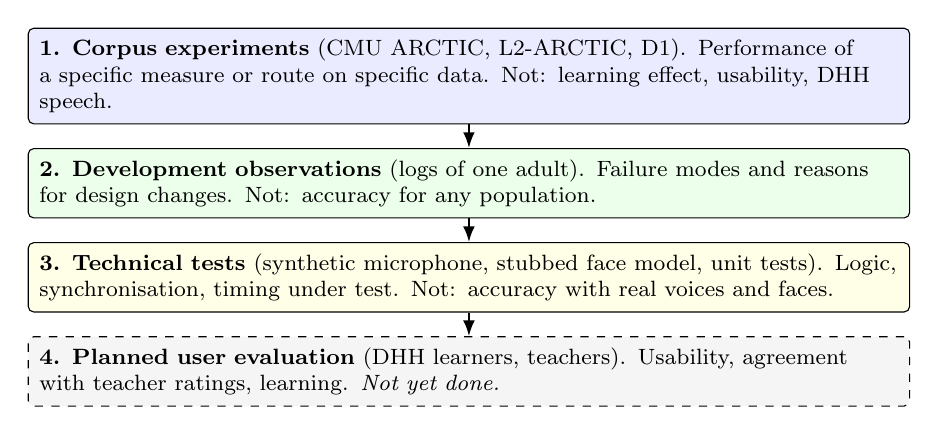
\begin{tikzpicture}[font=\footnotesize,
  tier/.style={draw, rounded corners=2pt, align=left, text width=0.9\columnwidth, inner sep=4pt},
  arr/.style={-{Latex[length=2mm]}, thick}]
  \node[tier, fill=blue!8] (t1) {\textbf{1. Corpus experiments} (CMU ARCTIC, L2-ARCTIC, D1). Performance of a specific measure or route on specific data. Not: learning effect, usability, DHH speech.};
  \node[tier, fill=green!8, below=3mm of t1] (t2) {\textbf{2. Development observations} (logs of one adult). Failure modes and reasons for design changes. Not: accuracy for any population.};
  \node[tier, fill=yellow!10, below=3mm of t2] (t3) {\textbf{3. Technical tests} (synthetic microphone, stubbed face model, unit tests). Logic, synchronisation, timing under test. Not: accuracy with real voices and faces.};
  \node[tier, dashed, fill=gray!8, below=3mm of t3] (t4) {\textbf{4. Planned user evaluation} (DHH learners, teachers). Usability, agreement with teacher ratings, learning. \emph{Not yet done.}};
  \draw[arr] (t1) -- (t2); \draw[arr] (t2) -- (t3); \draw[arr] (t3) -- (t4);
\end{tikzpicture}
\caption{Levels of evidence used in this paper and what each can support. Results from different levels are not combined.}
\label{fig:tiers}
\end{figure}

\section{Results}
\subsection{Summary for the Eight Sounds}
Table~\ref{tab:summary} lists, for each sound, the target words used in the experiments, the method that was evaluated, the accuracy on native speech, the behaviour on annotated learner speech, and the route that the learner application uses now. Two points should be noted. First, native accuracy is high for all sounds except \ipa{f}, for which only a weak hiss can be distinguished from the sibilants and the contrast with \ipa{\texttheta} is not established. Second, learner error counts are very small for \ipa{f}, \ipa{m}, \ipa{n}, and \ipa{t\textesh}, so that their detection rates are not interpretable.

\begin{table*}[!t]
\caption{Summary by sound. Native accuracy: balanced accuracy, leave-one-voice-out, ARCTIC. L2: L2-ARCTIC; FR = false rejection of correct productions, Det. = detection of annotated errors, percentages with Wilson 95\% intervals; $n$ = correct / error. ``Evaluated method'' is what these numbers were obtained with; ``Route now'' is the route of the current learner application (Section~\ref{sec:assess}), which has not been evaluated on L2-ARCTIC where it differs.}
\label{tab:summary}
\centering
\footnotesize
\begin{tabular}{lllcccl}
\toprule
Sound & Words evaluated & Evaluated method & Native acc. & L2 $n$ & L2 FR / Det. (\%) & Route now \\
\midrule
\ipa{s} & see, sip, sun & Recogniser identity + CoG/LDA degree & 0.95\textsuperscript{a} & 861 / 18 & 8 [6, 10] / 100 [82, 100] & Sustained hiss; word route \\
\ipa{\textesh} & she, ship, shoe & Recogniser identity + CoG/LDA degree & 0.95\textsuperscript{a} & 602 / 32 & 3 [2, 5] / 88 [72, 95] & Sustained hiss; word route \\
\ipa{f} & fee, fan, food & Recogniser identity + relative level & 0.93\textsuperscript{b} & 1160 / 1 & 11 [9, 13] / n/a (1 error) & Word route \\
\ipa{t\textesh} & cheat & Probe on hiss vs.\ \ipa{\textesh} & 0.96\textsuperscript{c} & 267 / 5 & 7 [5, 11] / 20 [4, 62] & GOP + two lamps \\
\ipa{m} & me & Recogniser at the nasal & 0.98\textsuperscript{d} & 1205 / 0 & 1 [1, 2] / n/a (0 errors) & GOP \\
\ipa{n} & knee & Recogniser at the nasal & 0.98\textsuperscript{d} & 682 / 3 & 1 [0, 2] / 33 [6, 79] & GOP \\
\ipa{p} & pea & Probe on release (VOT fallback) & 0.96\textsuperscript{e} & 309 / 86 & 36 [31, 41] / 85 [76, 91] & GOP \\
\ipa{b} & bee & Probe on release (VOT fallback) & 0.96\textsuperscript{e} & 962 / 26 & 10 [8, 12] / 54 [35, 71] & GOP \\
\bottomrule
\multicolumn{7}{l}{\scriptsize \textsuperscript{a}\ipa{s}--\ipa{\textesh}, calibrated, end-to-end (CoG alone: 0.87 uncalibrated, 0.93 normalised). \textsuperscript{b}weak hiss against sibilants, end-to-end; \ipa{f}--\ipa{\texttheta} not distinguished (0.67 on the hiss alone).} \\
\multicolumn{7}{l}{\scriptsize \textsuperscript{c}\ipa{t\textesh}--\ipa{\textesh}, end-to-end (hand-crafted features: 0.80). \textsuperscript{d}\ipa{m}--\ipa{n} (Praat formants: 0.63). \textsuperscript{e}\ipa{p}--\ipa{b} (VOT rule: 0.88 end-to-end).} \\
\end{tabular}
\end{table*}

\subsection{Agreement with Manual Measurement}
On D1, the CoG computed by the tool differed from the manual Praat values by less than 2~Hz, the automatic boundaries lay within 20~ms of the manual boundaries, and all six recordings were assigned to the correct sound. This agreement, however, concerns two dictionary voices only.

\begin{figure*}[!t]
\centering
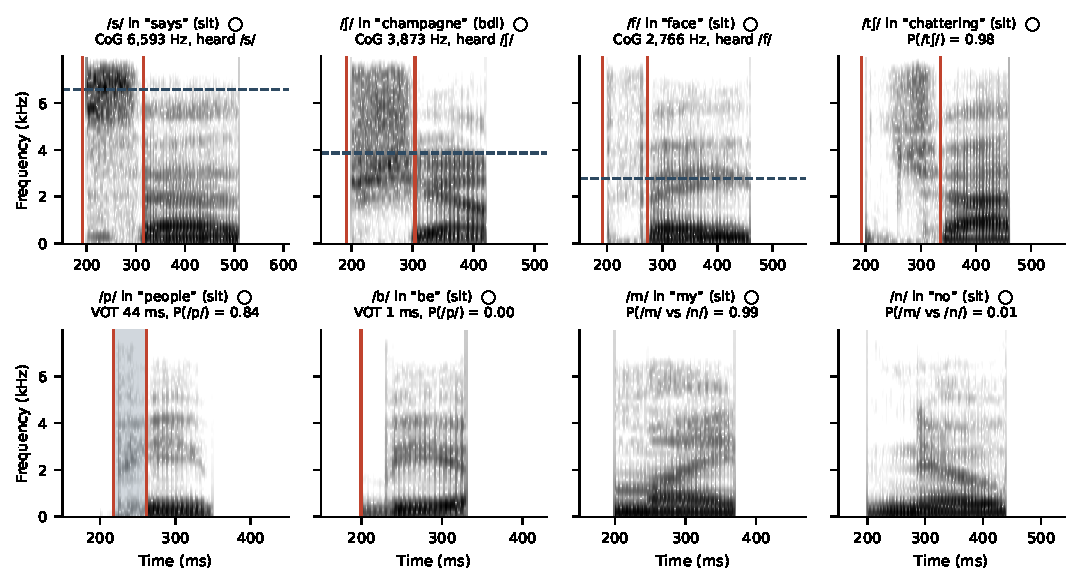
\includegraphics[width=\textwidth]{figs/fig_all_sounds.pdf}
\caption{Full spectrograms (0--8~kHz) of one correctly produced token of each of the eight sounds (native ARCTIC voices, sentences not used for training), cut like an isolated word, with what the tool detected at the time of the evaluation: red lines mark the detected hiss (fricatives, \ipa{t\textesh}) or the burst and the start of voicing (stops), the shaded area is the VOT interval, the dashed line is the CoG, and the title gives the verdict and the value on which it rests. For \ipa{m} and \ipa{n} the recogniser's probability is shown. Tokens were chosen as the first correct verdict for each sound, excluding a verdict resting on a mis-located hiss (see Section~\ref{sec:disc}).}
\label{fig:allsounds}
\end{figure*}

\begin{figure*}[!t]
\centering
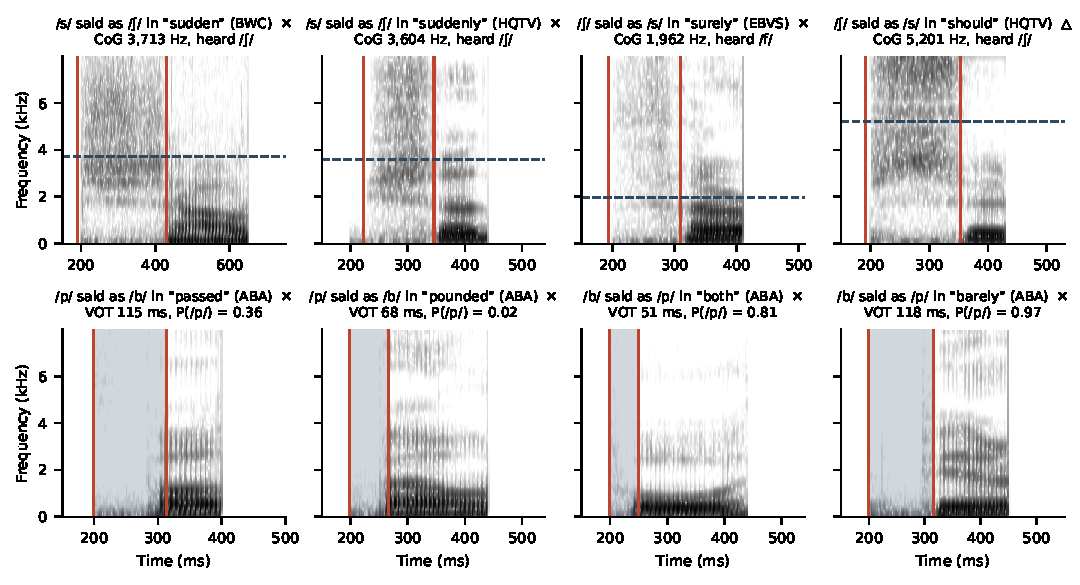
\includegraphics[width=\textwidth]{figs/fig_l2_errors.pdf}
\caption{Annotated learner substitutions in L2-ARCTIC and the verdict of the pipeline evaluated in this section. Top: \ipa{s} said as \ipa{\textesh} and the reverse (the last panel is a miss: the tool hears \ipa{\textesh} and gives \textit{almost}); bottom: \ipa{p} said as \ipa{b} and the reverse. In the first bottom panel the VOT is long (115~ms) although the annotators heard \ipa{b}, which is why a VOT rule alone fails.}
\label{fig:errors}
\end{figure*}

\begin{figure*}[!t]
\centering
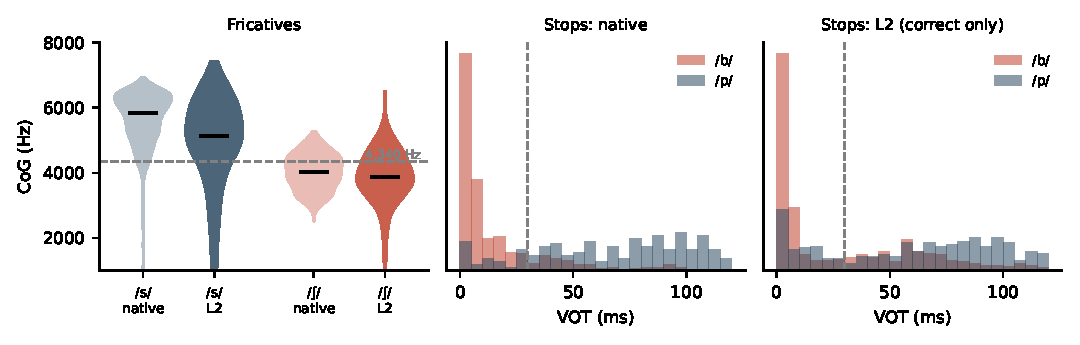
\includegraphics[width=0.92\textwidth]{figs/fig_shift.pdf}
\caption{Why native-voice rules fail for learners. Left: CoG of word-initial \ipa{s} and \ipa{\textesh} in native ARCTIC voices and in correctly produced L2 speech; the L2 \ipa{s} extends below the fixed 4{,}340~Hz threshold. Right: VOT of \ipa{p} and \ipa{b} in native and correctly produced L2 speech; the 30~ms threshold separates the learners' categories less well.}
\label{fig:shift}
\end{figure*}

\subsection{Population Shift: Native Thresholds on Learner Speech}
Table~\ref{tab:l2} and Fig.~\ref{fig:shift} show that the threshold rules, although accurate on D1, rejected 45\% of the correctly produced \ipa{s} and 43\% of the correctly produced \ipa{\textesh} of L2 speakers. The recogniser-assisted fricative route reduced these false rejections to 8\% and 3\%, respectively, and the annotated errors were retained at 100\% and 88\%. For the four Vietnamese speakers, the corresponding false-rejection rates were 7\% and 3\%, with 16/16 and 28/30 errors retained. It is concluded that, for these two sounds, native-voice thresholds are not sufficient, and that an additional decision on the identity of the sound is required.

\begin{table}[!htb]
\caption{Fricative errors in L2-ARCTIC: false rejection of correct productions (FR) and detection of annotated errors (Det.). Wilson 95\% intervals in brackets.}
\label{tab:l2}
\centering
\small
\begin{tabular}{llcc}
\toprule
Sound & Scoring & FR (correct) & Det. (errors) \\
\midrule
\multirow{2}{*}{\ipa{s}} & Thresholds & 45\% [42, 49] & 83\% [61, 94] \\
 & Recogniser-assisted & 8\% [6, 10] & 100\% [82, 100] \\
 & \scriptsize{$n$ (correct / error)} & \scriptsize{861} & \scriptsize{18} \\
\midrule
\multirow{2}{*}{\ipa{\textesh}} & Thresholds & 43\% [39, 47] & 84\% [68, 93] \\
 & Recogniser-assisted & 3\% [2, 5] & 88\% [72, 95] \\
 & \scriptsize{$n$ (correct / error)} & \scriptsize{602} & \scriptsize{32} \\
\bottomrule
\end{tabular}
\end{table}

\subsection{Stops}
For \ipa{p} and \ipa{b}, a fixed VOT threshold of 30~ms gave a balanced accuracy of 0.88 on native speech, but on L2 speech it was a weak detector (Table~\ref{tab:stops}). The probe trained on native speech (balanced accuracy 0.96, leave-one-voice-out) detected 85\% of the annotated \ipa{p} errors, most of which were \ipa{p} produced as \ipa{b}, compared with 43\% for the VOT rule, and it reduced the false-rejection rate of \ipa{b} from 39\% to 10\%. However, 36\% of the correctly annotated \ipa{p} were still rejected, and part of this may reflect weakly aspirated productions that the annotators accepted. The detection of \ipa{b} errors rests on 26 cases only. This probe is the version that was evaluated; the application now scores these sounds with the GOP route (Section~\ref{sec:gop}).

\begin{table}[!htb]
\caption{Stops in L2-ARCTIC: VOT rule versus recogniser probe.}
\label{tab:stops}
\centering
\small
\begin{tabular}{llcc}
\toprule
Sound & Scoring & FR (correct) & Det. (errors) \\
\midrule
\ipa{p} & VOT $\geq$ 30 ms & 28\% [24, 34] & 43\% [33, 54] \\
($n$ = 309 / 86) & Probe & 36\% [31, 41] & 85\% [76, 91] \\
\midrule
\ipa{b} & VOT $<$ 30 ms & 39\% [36, 42] & 46\% [29, 65] \\
($n$ = 962 / 26) & Probe & 10\% [8, 12] & 54\% [35, 71] \\
\bottomrule
\end{tabular}
\end{table}

\subsection{Context Leakage in Recogniser Evaluation}
When applied to whole words of eight native voices, the recogniser separated \ipa{f} from \ipa{\texttheta} with an accuracy of 0.99. Because the recogniser reads the entire clip, this figure may reflect the remainder of the word, and three controls were therefore applied. With the hiss alone, \ipa{f}--\ipa{\texttheta} accuracy fell to 0.67, whereas \ipa{s}--\ipa{\textesh} accuracy remained at 0.94. When the hiss of one sound was spliced into a word beginning with the other (320 splices per case), the recogniser followed the word rather than the hiss in 69--73\% of the \ipa{f}--\ipa{\texttheta} cases, but followed the hiss in 73--90\% of the \ipa{s}--\ipa{\textesh} cases. At a signal-to-noise ratio of 10~dB, \ipa{f}--\ipa{\texttheta} accuracy was 0.71. It follows that recogniser accuracy measured on words overstates its ability to discriminate the consonant itself for the \ipa{f}--\ipa{\texttheta} pair, and that this pair cannot currently be scored reliably from the hiss; it is therefore not graded.

\begin{figure}[!htb]
\centering
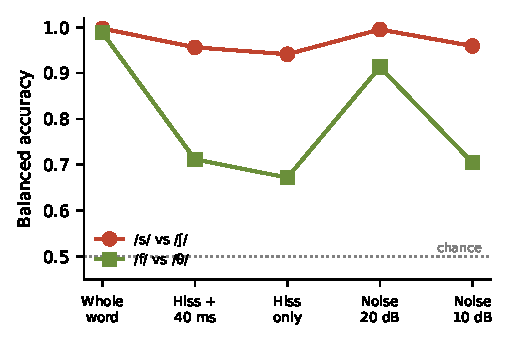
\includegraphics[width=0.85\columnwidth]{figs/fig_context.pdf}
\caption{Recogniser accuracy for \ipa{s}--\ipa{\textesh} and \ipa{f}--\ipa{\texttheta} as the context is removed or noise is added (eight native voices). The \ipa{f}--\ipa{\texttheta} contrast depends on the surrounding word.}
\label{fig:context}
\end{figure}

\subsection{Other Sounds and Personalisation}
For \ipa{m} and \ipa{n}, formant measures with Praat reached only 0.63 balanced accuracy on native speech, and the recogniser reached 0.98 on the words \textit{me} and \textit{knee}, which share the vowel and therefore do not reveal the answer through context. For \ipa{t\textesh} against \ipa{\textesh}, the recogniser probe reached 0.96 end-to-end (hand-crafted rise-time features: 0.80). Fewer than six annotated learner errors are available for \ipa{t\textesh}, \ipa{m}, \ipa{n}, and \ipa{f}, so that no error-detection rate is reported for them. For \ipa{s} against \ipa{\textesh}, per-speaker normalisation raised balanced accuracy from 0.90 to 0.97 across eight native voices, and six calibration recordings sufficed (0.95 end-to-end).

\subsection{Acoustic Cues for Live Guidance}
The live dot and the offline measure compute the CoG differently, so their zones were compared on 7{,}104 word-initial \ipa{s} and \ipa{\textesh} tokens of four adult voices (two male, two female) of CMU ARCTIC, using the labels of the corpus packages and a simulation of the browser analyser (Table~\ref{tab:cog}). The amplitude-weighted measure that the dot first used was the weakest (pooled AUC 0.76); a power-weighted CoG between 2 and 8~kHz reached 0.86, and the offline Praat-style measure 0.92. The midpoints between the two sounds differed by voice (3944 to 4748~Hz), which the voice-size factor is meant to absorb; this was not checked on these voices. The analysis concerns adult read speech at 16~kHz and the separation of \ipa{s} from \ipa{\textesh}, not the share of correct productions of the application. The thresholds were chosen on the same tokens, so the numbers are exploratory.

\begin{table}[!htb]
\caption{Separation of \ipa{s} and \ipa{\textesh} by three CoG measures (7{,}104 tokens, four adult ARCTIC voices, middle 60\% of each token).}
\label{tab:cog}
\centering
\small
\begin{tabular}{lcc}
\toprule
Measure & Pooled AUC & Per-voice AUC \\
\midrule
Amplitude-weighted, 1--8~kHz (first dot) & 0.76 & 0.71--0.89 \\
Power-weighted, 2--8~kHz (live, chosen) & 0.86 & 0.84--0.91 \\
Power-weighted, whole spectrum (offline) & 0.92 & 0.90--0.95 \\
\bottomrule
\end{tabular}
\end{table}

For \ipa{t\textesh}, two voices of ARCTIC (one male, one female; running speech) were used. The steepest rise of the hiss envelope separated \ipa{t\textesh} from \ipa{\textesh} with an AUC of 0.83 and 0.87, and the length of the hiss separated \ipa{t\textesh} from \ipa{t} with 0.89 and 0.91; the best limits differed clearly between the two voices, and the rise time itself and the CoG did not help. The limits used for the two lamps come from these figures and from ARCTIC words after a pause; they have not been checked on isolated \ipa{t\textesh} produced by learners.

\subsection{Development Observations of the GOP Route}
The GOP route was first tried on 53 recordings of one adult speaker made with the application (Table~\ref{tab:gop}). These counts show how the verdicts were distributed; they are not accuracies, because no independent label exists for these recordings. Three recordings of \textit{bee} that the speaker had flagged as wrongly judged \ipa{p} received $P(\mathrm{b})=0.98$, and seven of eight \textit{cheat} recordings had \ipa{t\textesh} as the top candidate. A second round with notes of the speaker's own trials showed errors of the recogniser that persist: \ipa{b} before \ipa{a}, \ipa{u}, or a schwa was often heard as \ipa{m}, and \ipa{m} before \ipa{u} as \ipa{n}. A second recogniser with the same vocabulary did not do better (the two agreed on the top sound in 43 of 60 recordings) and was dropped. \ipa{b}, \ipa{m}, and \ipa{n}, which all involve closed lips or nasal airflow, are the most difficult group in these data.

\begin{table}[!htb]
\caption{Verdicts of the GOP route on 53 development recordings of one adult speaker (not accuracy).}
\label{tab:gop}
\centering
\small
\begin{tabular}{lccccc}
\toprule
Sound & Correct & Almost & Not yet & Unsure & No speech \\
\midrule
\ipa{t\textesh} & 5 & 2 & 1 & 0 & 0 \\
\ipa{n} & 4 & 1 & 1 & 2 & 1 \\
\ipa{m} & 3 & 2 & 2 & 0 & 0 \\
\ipa{b} & 7 & 0 & 12 & 2 & 0 \\
\ipa{p} & 2 & 0 & 4 & 2 & 0 \\
\bottomrule
\end{tabular}
\end{table}

\subsection{Functional Checks}
The application has 86 automated tests for the scoring rules, the star and unlock rules, the quality gate, and the display zones; these are software checks and say nothing about the accuracy of pronunciation judgements. In addition, the lesson page was driven in a desktop browser with a synthetic microphone. A silent signal was refused with the message that the sound was too quiet and logged as such. A synthetic hiss held for about three seconds followed by a voiced vowel was judged as three stars through the sustained-fricative route, opened the next lesson, was written to the attempt log with its live summary, and did not trigger a second celebration at a second attempt. The smile bar of the lip mirror filled after about 480~ms of voice in a test with a stubbed face model, which matches the 0.5~s hold that is required; this is the accumulated hold time, not a delay of the display. The lip mirror was also switched on with the browser's fake camera, which contains no face, and showed the message that no face could be seen. All of this used synthetic input and does not show how well the guidance works with real voices and faces.

\section{Discussion and Limitations}\label{sec:disc}
The principal technical finding is that validation on native speech is not sufficient for an assistive pronunciation tool, because a measure that agrees with expert manual measurement can nevertheless reject a substantial share of correct learner productions. The context-controlled tests further show that the choice of evaluation unit influences the conclusion about a recogniser. In practical terms, a design in which the identity of the sound is decided by a recogniser and the degree of correctness by interpretable acoustic measures retains the visual transparency that DHH learners and teachers require.

The system design raises questions that the evaluations above do not answer. First, the three routes answer different questions. The sustained-fricative route tells whether the child completed a hold-the-hiss exercise; a short word produced correctly might not meet that requirement, and a green result does not show that the vowel followed correctly. The word and GOP routes judge a short word after the recording. A child may therefore see a live indicator and a later verdict that disagree (for example, the \ipa{t\textesh} lamps and the GOP verdict), and a policy for such conflicts is still to be decided. Second, the live dot is a weaker judge than the offline measure (AUC 0.86 against 0.92), and it separates \ipa{s} from \ipa{\textesh} wrongly about once in four attempts, so it is a guide for practice and not an assessment. Third, the recording rules differ between tasks: the word recorder stops after three seconds, while the guided recorders stop on silence or on completion of the task, and only the guided recorders listen to the room. Differences of this kind can affect the numbers in the log, and a single recording procedure would make recordings from different tasks and children easier to compare. Fourth, the camera can show only visible lip movements; it does not show the tongue, the airflow, or voicing, and for \ipa{p} and \ipa{b} the lip steps can be completed without any sound.

Several further limitations must be stated. No DHH learner has yet used the tool, and the L2 speakers of the corpus are hearing speakers; the findings therefore cannot be generalised to DHH speech, which may differ in pitch, intelligibility, and breathiness. All consonants in the corpus experiments were cut from continuous sentences, not recorded as isolated words. The annotated errors are few for several sounds, and the annotation reflects perceptual judgement by listeners, which may favour a recogniser trained on phonemic transcriptions. The thresholds and the displayed scores (GOP limits, lip ratios, hold durations, quality-gate limits, the pass line of two stars, and the voice-size factor) were set on small amounts of data, mainly from one adult, and the scores are model outputs, not calibrated probabilities. The recogniser branches require the model to be installed. The boundary detector can mislocate the hiss (for example, a \ipa{\textesh} in ``sure'' was measured at a CoG of 368~Hz), and in such a case the recogniser's decision, not the measurement, determines the verdict. The Chinese texts of the interface were written during development and have not been reviewed by a native-speaking educator. Finally, learning outcomes have not been measured, and stars and the lesson order are application rules, not evidence of mastery.

\section{Planned User Evaluation}
The planned evaluation has several strands with different questions.

\subsection{Expert Review}
Phoneticians, speech-language pathologists, and teachers of DHH learners review the articulation illustrations, the lip steps, the tips, the order of the lessons, and the meaning of the three-level feedback \tbd{number and recruitment of experts}.

\subsection{Teacher Strand}
Teachers of English or speech-language specialists who work with DHH learners are invited \tbd{number, recruiting site, years of experience}. After a short demonstration, each teacher uses the tool with the eight target words and then completes a short questionnaire on the clarity of the three-level verdict and of the live displays and on the usefulness of the measures and tips \tbd{items, scale, source of any adapted instrument}. Open comments are coded thematically \tbd{coding procedure}.

\subsection{Learner Strand}
Learners record the eight target words \tbd{population: hearing EFL learners first; DHH learners, including children with cochlear implants, conditional on ethical approval and consent; number, age range}. At least two teachers, blind to the tool's verdicts, rate each target consonant as correct, almost, or not yet \tbd{scale, rater training, number of raters}. Agreement between the tool and the teachers is compared with agreement between the teachers \tbd{statistic, e.g., weighted kappa}, separately for each assessment route and with the unscored attempts reported. Usability measures include the completion of each step, the help needed, and the understanding of the colours. Learning outcomes (pre/post, retention, and transfer to untrained words) belong to a later stage.

\subsection{Ethics}
\tbd{ethical approval number, informed consent for adults, parental consent and child assent where learners are minors, data storage and anonymisation}.

\section{Conclusion}
SeeSound, a prototype with a learner interface and a researcher/teacher interface for eight English consonants, was described and evaluated technically. On annotated learner speech, thresholds validated on native voices over-rejected correct productions, whereas a recogniser-assisted route reduced false rejection for \ipa{s} and \ipa{\textesh} to 8\% and 3\% without losing the annotated confusions; a live CoG indicator separated the two sounds with an AUC of 0.86; and the \ipa{f}--\ipa{\texttheta} contrast could not be established from the consonant alone. The GOP and sustained-fricative routes have been tested for function but not against independent labels. The prototype is intended to support independent practice by DHH children after initial guidance and educator-led intervention; whether it does so remains to be shown. Future work comprises recording isolated words from native, L2, and DHH speakers, evaluating each route against independent ratings, reviewing the content with experts, and measuring usability and the effect of the feedback on learning.

\section*{Acknowledgment}
\tbd{Funding and acknowledgements (FTIP project, National Formosa University).}

\begin{thebibliography}{00}
% Entries marked "checked" were compared with Crossref, ISCA, or publisher records on 2026-11-03 (author order, pages, DOI). The others (truong2005, moradi2017, desai2008, winn2013, pimperton2017, ertmer2011, kim2025, kuperman2012) have not been re-checked in this revision. A reference to Carroll et al. (ESSV 2015), whose details could not be verified, was removed.
\bibitem{ertmer2011} D. J. Ertmer and L. Goffman, ``Speech production accuracy and variability in young cochlear implant recipients: Comparisons with typically developing age-peers,'' \textit{J. Speech Lang. Hear. Res.}, vol. 54, no. 1, pp. 177--189, 2011.
\bibitem{stelmachowicz2004} P. G. Stelmachowicz, A. L. Pittman, B. M. Hoover, D. E. Lewis, and M. P. Moeller, ``The importance of high-frequency audibility in the speech and language development of children with hearing loss,'' \textit{Arch. Otolaryngol. Head Neck Surg.}, vol. 130, no. 5, pp. 556--562, 2004, doi: 10.1001/archotol.130.5.556.
\bibitem{hitchcock2023} E. R. Hitchcock, L. C. Ochs, M. T. Swartz, M. C. Leece, J. L. Preston, and T. McAllister, ``Tutorial: Using visual--acoustic biofeedback for speech sound training,'' \textit{Am. J. Speech-Lang. Pathol.}, vol. 32, no. 1, pp. 18--36, 2023, doi: 10.1044/2022\_AJSLP-22-00142.
\bibitem{bu2021} Y. Bu \textit{et al.}, ``PTeacher: A computer-aided personalized pronunciation training system with exaggerated audio-visual corrective feedback,'' in \textit{Proc. CHI Conf. Human Factors in Computing Systems (CHI '21)}, 2021, pp. 1--14, doi: 10.1145/3411764.3445490.
\bibitem{neri2006} A. Neri, C. Cucchiarini, and H. Strik, ``ASR-based corrective feedback on pronunciation: Does it really work?'' in \textit{Proc. Interspeech}, 2006, doi: 10.21437/Interspeech.2006-543.
\bibitem{moradi2017} S. Moradi, B. Lidestam, H. Danielsson, E. H. N. Ng, and J. R{\"o}nnberg, ``Visual cues contribute differentially to audiovisual perception of consonants and vowels in improving recognition and reducing cognitive demands in listeners with hearing impairment using hearing aids,'' \textit{J. Speech Lang. Hear. Res.}, vol. 60, pp. 2687--2703, 2017.
\bibitem{desai2008} S. Desai, G. Stickney, and F.-G. Zeng, ``Auditory-visual speech perception in normal-hearing and cochlear-implant listeners,'' \textit{J. Acoust. Soc. Am.}, vol. 123, no. 1, pp. 428--440, 2008.
\bibitem{winn2013} M. B. Winn, A. E. Rhone, M. Chatterjee, and W. J. Idsardi, ``The use of auditory and visual context in speech perception by listeners with normal hearing and listeners with cochlear implants,'' \textit{Front. Psychol.}, vol. 4, art. 824, 2013.
\bibitem{pimperton2017} H. Pimperton, A. Ralph-Lewis, and M. MacSweeney, ``Speechreading in deaf adults with cochlear implants: Evidence for perceptual compensation,'' \textit{Front. Psychol.}, vol. 8, art. 106, 2017.
\bibitem{yang2017} J. Yang, J. Vadlamudi, Z. Yin, C.-Y. Lee, and L. Xu, ``Production of word-initial fricatives of Mandarin Chinese in prelingually deafened children with cochlear implants,'' \textit{Int. J. Speech-Lang. Pathol.}, vol. 19, no. 2, pp. 153--164, 2017, doi: 10.3109/17549507.2016.1143972.
\bibitem{ertmermaki2000} D. J. Ertmer and J. E. Maki, ``A comparison of speech training methods with deaf adolescents: Spectrographic versus noninstrumental instruction,'' \textit{J. Speech Lang. Hear. Res.}, vol. 43, no. 6, pp. 1509--1523, 2000, doi: 10.1044/jslhr.4306.1509.
\bibitem{ertmer2004} D. J. Ertmer, ``How well can children recognize speech features in spectrograms? Comparisons by age and hearing status,'' \textit{J. Speech Lang. Hear. Res.}, vol. 47, no. 3, pp. 484--495, 2004, doi: 10.1044/1092-4388(2004/038).
\bibitem{truong2005} K. Truong, A. Neri, F. de Wet, C. Cucchiarini, and H. Strik, ``Automatic detection of frequent pronunciation errors made by L2-learners,'' in \textit{Proc. Interspeech}, 2005.
\bibitem{kim2025} S.-E. Kim, B. R. Chernyak, J. Keshet, M. Goldrick, and A. R. Bradlow, ``Predicting relative intelligibility from inter-talker distances in a perceptual similarity space for speech,'' \textit{Psychon. Bull. Rev.}, vol. 32, pp. 1664--1675, 2025.
\bibitem{baevski2020} A. Baevski, Y. Zhou, A. Mohamed, and M. Auli, ``wav2vec 2.0: A framework for self-supervised learning of speech representations,'' in \textit{Advances in Neural Information Processing Systems}, vol. 33, 2020, pp. 12449--12460.
\bibitem{xu2022} Q. Xu, A. Baevski, and M. Auli, ``Simple and effective zero-shot cross-lingual phoneme recognition,'' in \textit{Proc. Interspeech}, 2022, pp. 2113--2117, doi: 10.21437/Interspeech.2022-60.
\bibitem{jongman2000} A. Jongman, R. Wayland, and S. Wong, ``Acoustic characteristics of English fricatives,'' \textit{J. Acoust. Soc. Am.}, vol. 108, no. 3, pp. 1252--1263, 2000, doi: 10.1121/1.1288413.
\bibitem{zhao2018} G. Zhao \textit{et al.}, ``L2-ARCTIC: A non-native English speech corpus,'' in \textit{Proc. Interspeech}, 2018, pp. 2783--2787, doi: 10.21437/Interspeech.2018-1110.
\bibitem{kuperman2012} V. Kuperman, H. Stadthagen-Gonzalez, and M. Brysbaert, ``Age-of-acquisition ratings for 30,000 English words,'' \textit{Behav. Res. Methods}, vol. 44, pp. 978--990, 2012.
\bibitem{kominek2004} J. Kominek and A. W. Black, ``The CMU Arctic speech databases,'' in \textit{Proc. 5th ISCA Workshop on Speech Synthesis (SSW 5)}, 2004, pp. 223--224.
\end{thebibliography}

\end{document}
